\documentclass[a4paper,12pt]{article}
\usepackage[margin=.9in]{geometry}
\usepackage{graphicx}
\usepackage{parskip}
\usepackage[utf8]{inputenc}
\usepackage{tikz}
\usetikzlibrary{shapes.geometric, arrows}
\graphicspath{ {images/} }
\usepackage{amsmath}
\usepackage{hyperref}

\newcommand{\mybox}[2]{{\color{#1}\fbox{\normalcolor#2}}}

\tikzstyle{module} = [rectangle, rounded corners, minimum width=2cm, minimum height=1.2cm,text centered, draw=black, fill=red!30, text width=3.5cm]

\tikzstyle{startstop} = [rectangle, rounded corners, minimum width=1.5cm, minimum height=.8cm,text centered, draw=black, fill=red!30]
\tikzstyle{io} = [trapezium, trapezium left angle=70, trapezium right angle=110, minimum width=1cm, minimum height=.8cm, text centered, draw=black, fill=blue!30, inner sep=.2cm]
\tikzstyle{process} = [rectangle, minimum width=3cm, minimum height=.8cm, text centered, draw=black, fill=orange!30, text width=3.5cm]
\tikzstyle{decision} = [diamond, minimum width=3cm, minimum height=.8cm, text centered, draw=black, fill=green!30, text width=1.8cm, aspect=1.8, inner sep=0]
\tikzstyle{arrow} = [thick,->,>=stealth]

\begin{document}
\begin{titlepage}
    \begin{center}
        \vspace*{1cm}
        
        \Huge
        \textbf{Technical Specification}
        
        \vspace{0.5cm}
        \LARGE
        SDP Group 15-H
        
        \vspace{1.5cm}
        \normalsize
		Emilia Bogdanova\\
		Patrick Green\\
        Julijonas Kikutis\\ 
		David McArthur\\
		Aseem Narang\\
		Ankit Sonkar\\
        
        \vfill
        
        
        \vspace{0.8cm}
        
        \begin{figure}
    	\vspace*{-2.5em}
    	\centering
    	
\includegraphics[scale=.30]{logo.png}
		\end{figure}
        
        \Large
        The University of Edinburgh\\
        
    \end{center}
\end{titlepage}

\tableofcontents

\newpage

\section{System architecture}

\section{Hardware components}

\subsection{Motors}

\subsection{Chassis Structure}

\subsection{Holonomics}
\begin{figure}
\centering
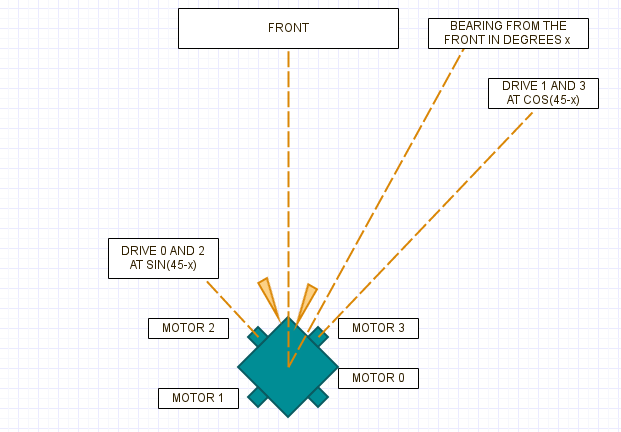
\includegraphics[scale=.5]{holonomics.png}
\caption{Visualisation of the calculating the motor power components}
\label{fig:components}
\end{figure}

Holonomic motion was an obvious choice for the final robot. It enabled fast motion in any direction meaning the robot could respond very  to a change in play. It also was perfectly suited to a strategy using potential fields as an optimal direction would be output and implemented instantly using the firmware. The motion was constructed by calculating the angle between the desired direction  and the robot orientation. This was used to compute the driving components that are sent to the Arduino as seen in Figure \ref{fig:components}. The matrix multiplication below was used to extract the driving powers and then each power was scaled up by a factor of $100$ divided by the absolute maximum of the four motor powers.

$$\begin{pmatrix}
\text{MOTOR 0}\\ 
\text{MOTOR 1}\\ 
\text{MOTOR 2}\\ 
\text{MOTOR 3}
\end{pmatrix}=
\begin{pmatrix}
1 & 0\\ 
0 & -1\\ 
-1 & 0\\ 
0 & 1 
\end{pmatrix}
\begin{pmatrix}
\cos(45-x)\\ 
\sin(45-x)
\end{pmatrix}$$

\subsection{Weight Distribution}

\subsection{Grabber}
The grabber consists of two symmetric parts placed one slightly above the other. To keep the robot within dimensions the grabber arms overlap enabling a large span but still within regulations when closed. A symmetric gear system is used so that both arms are opened and closed at the same time. Unlike the original design, the arm axles were placed closer together so that the grabbed ball would always be in the same position increasing the reliability of the sensor and the kick.

\subsection{Kicker}

%(Figure \ref{fig:kick_action}). 
%\begin{figure}
%    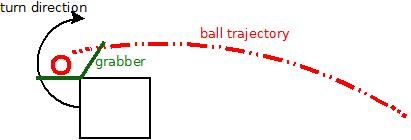
\includegraphics[scale=.7]{kick}
%    \caption{High level diagram of how the kick is performed}
%    \label{fig:kick_action}
%\end{figure}\newline

\begin{figure}[ht!]
\begin{minipage}{0.5\textwidth}
\centering
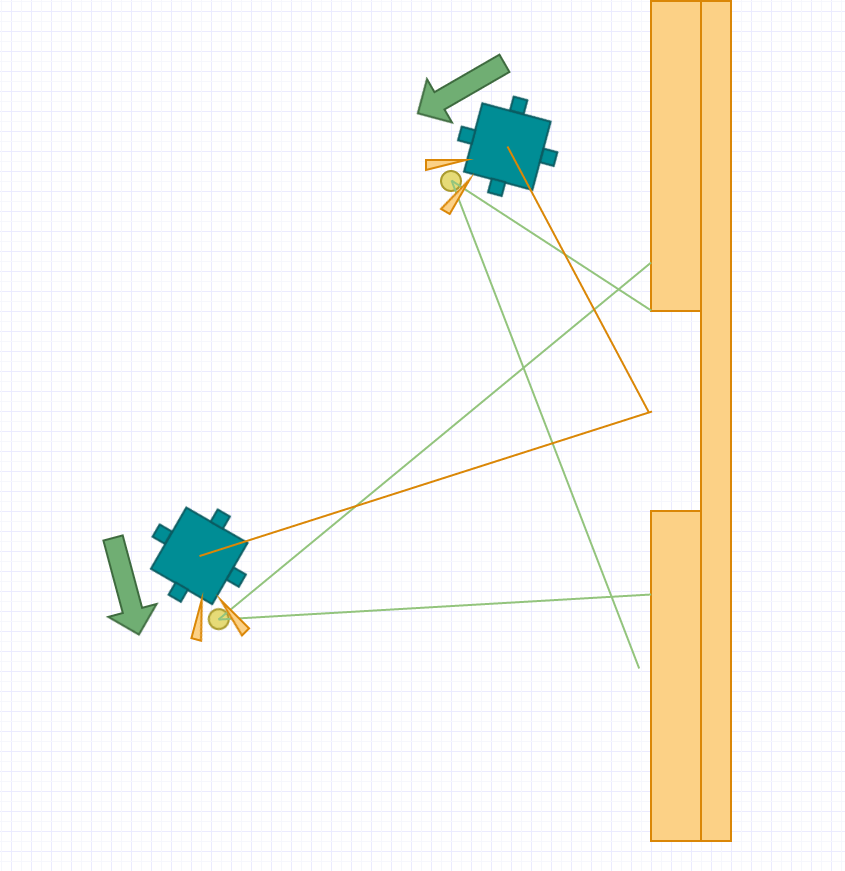
\includegraphics[width=80mm,height=100mm]{goodkick.png}
\caption{Correct kick rotation}
\label{fig:correct}
\end{minipage}
~
\begin{minipage}{0.5\textwidth}
\centering
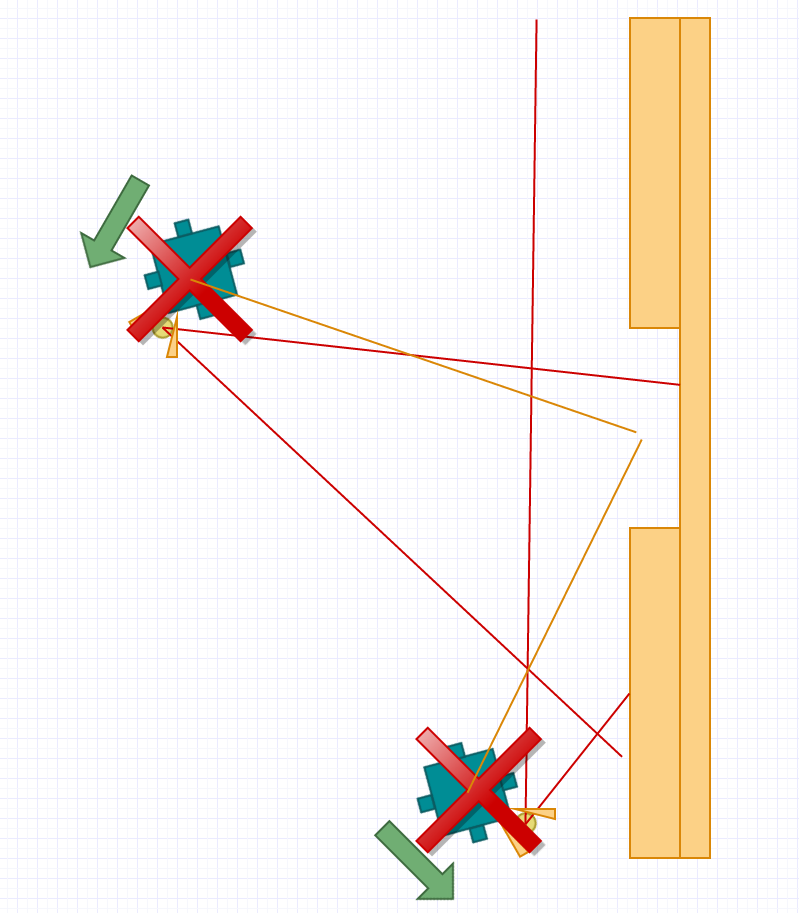
\includegraphics[width=75mm,height=100mm]{badkick.png}
\caption{Incorrect kick rotation}
\label{fig:incorrect}
\end{minipage}
\end{figure}

Our newest design does not have a kicker. The kick is made by turning the robot instead and opening the grabber at the same time. The main incentive of this design was to reduce asymmetric weight distribution which would have been catastrophic to optimising the holonomic movement. The robot rotates in the intended kick direction when it is aligning itself with the goal. In doing this the centrifugal force holds the ball towards the end of the grabber and the ball is in contact with the claw that will apply the kicking force. This increases the accuracy of the kick. As the error margin of the kick is asymmetric and biased towards undershooting, the kick is initiated in different directions in different positions on the pitch. The $y$ dimension is split into four segments: $0$, $\frac{1}{4}$, $\frac{1}{2}$, and $\frac{3}{4}$. In Figures \ref{fig:correct} and \ref{fig:incorrect} the robots demonstrate each segment and its correct and incorrect kick directions. This kicking mechanism is not only more powerful than the previous design but it is also able to confuse the defence strategies of opponents tournament\footnote{Footage of one such example of a confusing spin kick is available at \url{https://youtu.be/VJLo2x2gdGk}.}.


\section{Documentation of the code}

\begin{figure}[ht!]
\centering
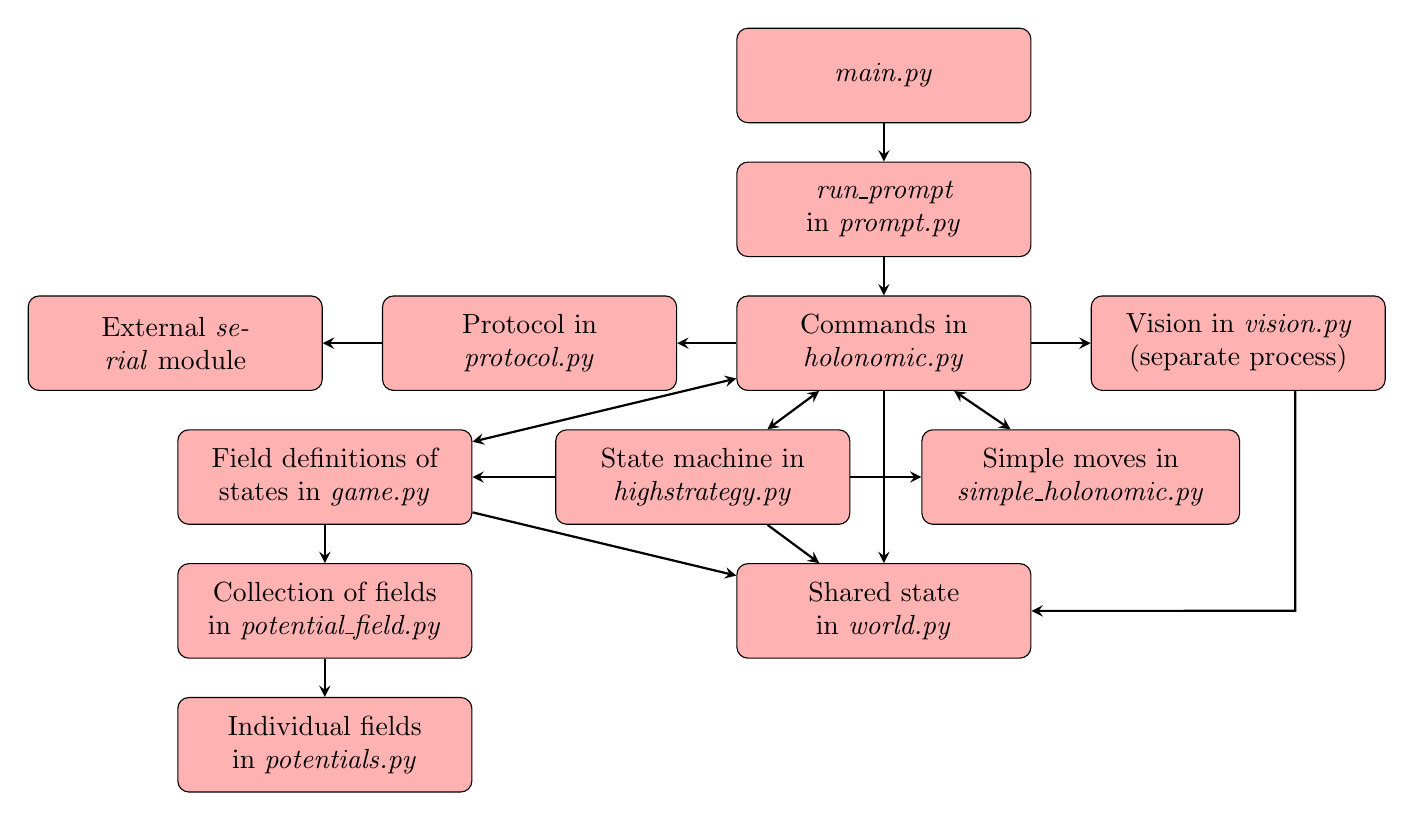
\begin{tikzpicture}[node distance=1.7cm]

\node (main) [module] {\textit{main.py}};
\node (prompt) [module, below of=main] {\textit{run\_prompt} in \textit{prompt.py}};
\draw [arrow] (main) -- (prompt);
\node (commands) [module, below of=prompt] {Commands in \textit{holonomic.py}};
\draw [arrow] (prompt) -- (commands);
\node (protocol) [module, left of=commands, xshift=-2.8cm] {Protocol in \textit{protocol.py}};
\draw [arrow] (commands) -- (protocol);
\node (serial) [module, left of=protocol, xshift=-2.8cm] {External \textit{serial} module};
\draw [arrow] (protocol) -- (serial);

\node (world) [module, below of=commands, yshift=-1.7cm] {Shared state in \textit{world.py}};
\draw [arrow] (commands) -- (world);

\node (vision) [module, right of=commands, xshift=2.8cm] {Vision in \textit{vision.py} (separate process)};
\draw [arrow] (commands) -- (vision);
\draw [arrow] (vision.320) |- ++(0, -2.792cm) -- (world);

\node (moves) [module, below of=commands, xshift=2.5cm, text width=3.8cm] {Simple moves in \textit{simple\_holonomic.py}};
\draw [arrow, <->] (commands) -- (moves);

\node (state) [module, below of=commands, xshift=-2.3cm] {State machine in \textit{highstrategy.py}};
\draw [arrow, <->] (commands) -- (state);
\draw [arrow] (state) -- (moves);
\draw [arrow] (state) -- (world);

\node (game) [module, below of=commands, xshift=-7.1cm] {Field definitions of states in \textit{game.py}};
\draw [arrow, <->] (commands) -- (game);
\draw [arrow] (state) -- (game);
\draw [arrow] (game) -- (world);
\node (field) [module, below of=game] {Collection of fields in \textit{potential\_field.py}};
\draw [arrow] (game) -- (field);
\node (pot) [module, below of=field] {Individual fields in \textit{potentials.py}};
\draw [arrow] (field) -- (pot);

\end{tikzpicture}
\caption{Dependency graph of Python modules in the system}
\label{fig:overview}
\end{figure}

The code is subdivided into several Python modules as seen in Figure \ref{fig:overview}. The module \textit{main} is used to launch the \textit{prompt} module. The commands in the prompt are provided by the \textit{commands} module. It creates instances of protocol, vision, and state machine objects from the respective modules. The vision object is run on a separate thread to process frames asynchronously with constantly updated shared world state kept in a \textit{World} object. At the same time the prompt is provided for the user. The command to run the strategy is called \texttt{hs}. This command constantly queries the state machine in the \textit{highstrategy} module. The state machine checks the world state to decide which state it is currently in and then performs the associated action. It is done either by handing over the execution to \textit{game} module to construct a potential field and perform the best action based on it or performing a predefined move from the \textit{simple\_holonomic} module.

All code except the color calibration user interface in the \textit{vision} module is an original work. Libraries used are \textit{pyserial}, \textit{numpy}, \textit{scipy}, and \textit{OpenCV}.

\subsection{Communications}

The communication interface between the Arduino and PC is low level as the PC decides and specifies the individual motor numbers and rotary encoder value or time duration for which they will be powered. Then the Arduino sends acknowledgement to the PC about the arrival of the command, turns the motors on, and sets the specified timeouts to stop them. The messages are human-readable, newline-terminated and tokens inside them are separated by spaces. The specified motor power can be negative, in which case it means backwards direction. Each message which changes the state of the robot has a sequence number and checksum that are checked in the Arduino. The messages used in the protocol are listed in Table \ref{tab:messages}. The communication messages are constructed in the \textit{Protocol} class using methods named after the corresponding message in \texttt{control/protocol.py} and these are used in the motion commands in \texttt{control/holonomic.py}.

\begin{table}[h!]
\centering
\begin{tabular}{ | l | l | }
    \hline
    Rotate the motors for $n$ ms &
    \small{\texttt{M seqNo checksum n motorNo power...}} \\ \hline
    Rotate the motors for $n$ rotary values &
    \small{\texttt{R seqNo checksum n motorNo power...}} \\ \hline
    Rotate the motors indefinitely &
    \small{\texttt{V seqNo checksum motorNo power...}} \\ \hline
    Stop all motors &
    \small{\texttt{S seqNo checksum}} \\ \hline
    Return \texttt{D} if all motors are stopped &
    \small{\texttt{I}} \\ \hline
    Handshake, reset the sequence number &
    \small{\texttt{H}} \\ \hline
    Query light sensor, return \texttt{D} or \texttt{N} &
    \small{\texttt{A threshold}} \\ \hline
    Transfer a byte to I2C bus &
    \small{\texttt{T byteInDecimalASCII}} \\ \hline
\end{tabular}
\caption{Messages available in the protocol}
\label{tab:messages}
\end{table}

\subsection{Arduino}

\begin{figure}[ht!]
\centering
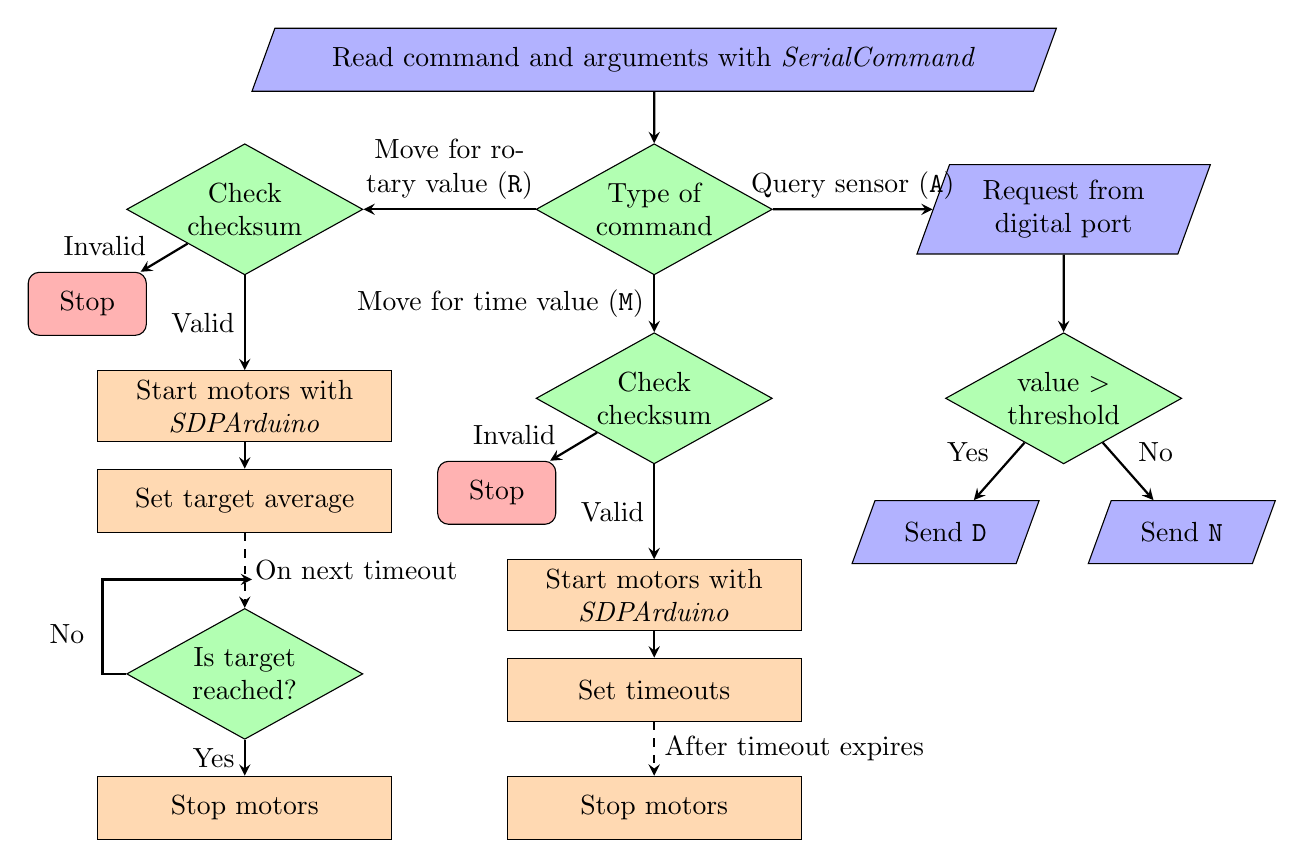
\begin{tikzpicture}[node distance=1.2cm]

\node (inCmd) [io] {Read command and arguments with \textit{SerialCommand}};
\node (decType) [decision, below of=inCmd, yshift=-.7cm] {Type of command};
\draw [arrow] (inCmd) -- (decType);

\node (decCheck1) [decision, left of=decType, xshift=-4cm] {Check checksum};
\draw [arrow] (decType) -- node [anchor=south, text width=3cm, text centered] {Move for rotary value (\texttt{R})} (decCheck1);
\node (stop1) [startstop, below of=decCheck1, xshift=-2cm] {Stop};
\draw [arrow] (decCheck1) -- node [anchor=south east, yshift=-.1cm, xshift=-.1cm] {Invalid} (stop1);
\node (motors1) [process, below of=decCheck1, yshift=-1.3cm, text width=3.5cm] {Start motors with \textit{SDPArduino}};
\draw [arrow] (decCheck1) -- node [anchor=east] {Valid} (motors1);
\node (target) [process, below of=motors1] {Set target average};
\draw [arrow] (motors1) -- (target);
\node (decTarget) [decision, below of=target, yshift=-1cm] {Is target reached?};
\draw [arrow, dashed] (target) -- node [anchor=west] {On next timeout} (decTarget);
\draw [arrow] (decTarget.west) |- node [anchor=east, xshift=-.4cm, yshift=.5cm] {No} ++(-.3cm, 0)
                               |- ++(0, 1.2cm)
                               -- ++(1.9cm, 0);
\node (stopMotors1) [process, below of=decTarget, yshift=-.5cm] {Stop motors};
\draw [arrow] (decTarget) -- node [anchor=east] {Yes} (stopMotors1);


\node (decCheck2) [decision, below of=decType, yshift=-1.2cm] {Check checksum};
\draw [arrow] (decType) -- node [anchor=east] {Move for time value (\texttt{M})} (decCheck2);
\node (stop2) [startstop, below of=decCheck2, xshift=-2cm] {Stop};
\draw [arrow] (decCheck2) -- node [anchor=south east, yshift=-.1cm, xshift=-.1cm] {Invalid} (stop2);
\node (motors2) [process, below of=decCheck2, yshift=-1.3cm, text width=3.5cm] {Start motors with \textit{SDPArduino}};
\draw [arrow] (decCheck2) -- node [anchor=east] {Valid} (motors2);
\node (timeouts) [process, below of=motors2] {Set timeouts};
\draw [arrow] (motors2) -- (timeouts);
\node (stopMotors2) [process, below of=timeouts, yshift=-.3cm] {Stop motors};
\draw [arrow, dashed] (timeouts) -- node [anchor=west] {After timeout expires} (stopMotors2);

\node (req) [io, right of=decType, xshift=4cm, text width=2.5cm] {Request from digital port};
\draw [arrow] (decType) -- node [anchor=south, text width=3cm, text centered] {Query sensor (\texttt{A})} (req);
\node (decComp) [decision, below of=req, yshift=-1.2cm] {value $>$ threshold};
\draw [arrow] (req) -- (decComp);
\node (sendD) [io, below of=decComp, xshift=-1.5cm, yshift=-.5cm] {Send \texttt{D}};
\draw [arrow] (decComp) -- node [anchor=south east] {Yes} (sendD);
\node (sendN) [io, below of=decComp, xshift=1.5cm, yshift=-.5cm] {Send \texttt{N}};
\draw [arrow] (decComp) -- node [anchor=south west] {No} (sendN);

\end{tikzpicture}
\caption{Flowchart of message processing in the Arduino}
\label{fig:flow}
\end{figure}

The Arduino code uses the \textit{SerialCommand} library to buffer and tokenize the commands received over the serial link. Messages changing the world state are sent with a sequence number and checksum which is the sum of all the parameters following it. If the sequence number matches the one from the last command, acknowledgement is sent but no further work is performed for the duplicate message. This handles the situation arising when an acknowledgement from the Arduino does not reach the PC and and the PC generates a duplicate message. If the checksum does not match, the Arduino code ignores the message and does not send an acknowledgement, thus forcing the PC to send the same message again.

If any of the motor move commands are sent, the motors are started immediately using the \textit{SDPArduino} library. Then the Arduino schedules when to stop the motors and there are two methods to perform that: either a time value or rotary encoder value. The flowchart for these two methods, along with querying the light sensor, are detailed in Figure \ref{fig:flow}.
In the case of the time value, a timeout is set to stop each single motor using
\textit{setTimeout} from the \textit{SimpleTimer} library.
In the case of rotary encoder value, \textit{setInterval} is used which calls
a function every 5 ms that queries the rotary encoder board and stops the motors
when the average of all four motor rotary encoder values reaches the target value. These approaches using timers
allows the robot to receive commands asynchronously, that is, a command is not
blocking during its execution and the PC software could, for example, send another command simultaneously to engage the kicker while the robot is in motion.
The Arduino message handling is located in \texttt{arduino/arduino.ino} file.

A buffer of upcoming motor jobs has also been implemented in the Arduino code to ensure continuous motion but it was deemed unnecessary as vision could issue new commands quickly enough without the robot coming to halt. The current implementation also never stops a motor when a new command arrives for the same motor, instead it just executes the new command, ensuring continuous motion.

\subsection{Vision}

In order to detect the robots and ball the following steps are executed:

\begin{enumerate}
\item The dictionary of the camera capture settings (brightness, contrast, hue and saturation) are read from \texttt{room0/1.txt}, pitch dimensions from \texttt{pitch0/1.txt}, and color thresholds from \texttt{color0/1.txt}.
\item The aforementioned settings are used, a frame is read, and the Gaussian blur is applied to create more solid features.
\item A unique application to speed up the feed is the variable \texttt{world.undistort} which lets the strategy to conditionally remove the barrel distortion when it is unnecessary.
\item All color thresholds are added to the same mask and K-means is used to group them together to form various spots in the image.
\item Then the color is found from the center pixel of the cluster. The spot is either kept or removed depending on the minimum area for that color which varies as some colors are more difficult to see.
\item The individual methods required for finding the robots and ball are then implemented as outlined below.
\item When the vision system is closed using the escape key, the most recent calibration values and the current camera settings defined by the slider bars are saved and can be used on the next execution.
\end{enumerate}

\subsubsection{Finding the robots}

Due to the varying light intensities over the pitch a highly tolerant method of identifying robots is used. The robot identities are pre-defined and dependent on the choice of the center and corner spot as seen in Figure \ref{fig:robots}. Numbers are assigned sequentially to our robot, teammate, first enemy, and second enemy.

\begin{figure}
\centering
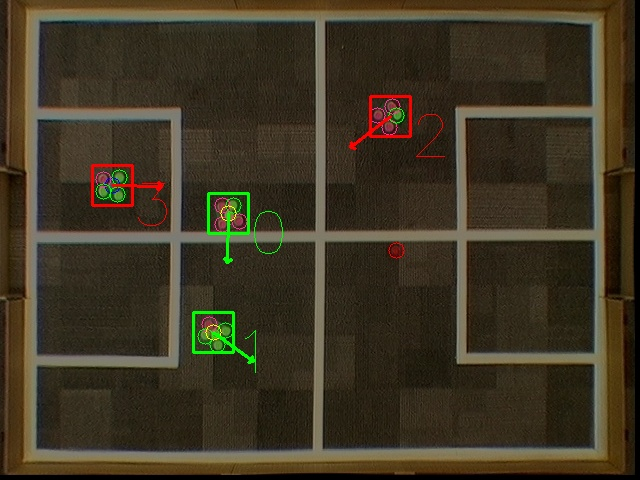
\includegraphics[height=40mm,width=60mm]{ex1.jpg}
\caption{The four robots marked on the vision feed.}
\label{fig:robots}
\end{figure}

There are two independent ways the robot can be identified:

\begin{minipage}{0.2\textwidth}
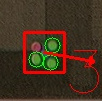
\includegraphics[scale=0.7]{3spot.jpg}
\end{minipage}
\begin{minipage}{0.8\textwidth}   
\textbf{The three spot method}: Finds the largest of the three distances between spots, then draws a vector from the midpoint of this edge to the spot not included in the edge. The orientation is then computable by rotating this vector by a fixed amount. Then, the robot center is calculated using the average of the spot centres.
\end{minipage}

\begin{minipage}{0.2\textwidth}
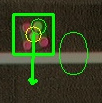
\includegraphics[scale=0.7]{2spot.jpg}
\end{minipage}
\begin{minipage}{0.8\textwidth}
\textbf{The two spot method}: As each spot is distinguishable, a vector can be constructed between the center spot and the corner spot and rotated a fixed amount to find the orientation. Then, the robot center is calculated using the center spot. 
\end{minipage}

\medskip

As there will always be two robots with the same plate configuration required for the methods above, the algorithm needs some of the robots to be identified using more information. As seen above, the robots from the same teams will have the same two spot plate configuration. Also, for the three spot method the robots 0, 2 and 1, 3 will have the same plate configurations. To solve this, the spots are initially grouped together into potential robots in the order of descending areas. The groups are run through several filters for each type of robot accepting the groups if there exists a specific numbers of coloured spots. Each spot that is found is circled with its respective color on the vision feed. The sets of spots on the filers bellow correspond to finding the robot zero.

\medskip

\begin{minipage}{0.6\textwidth}
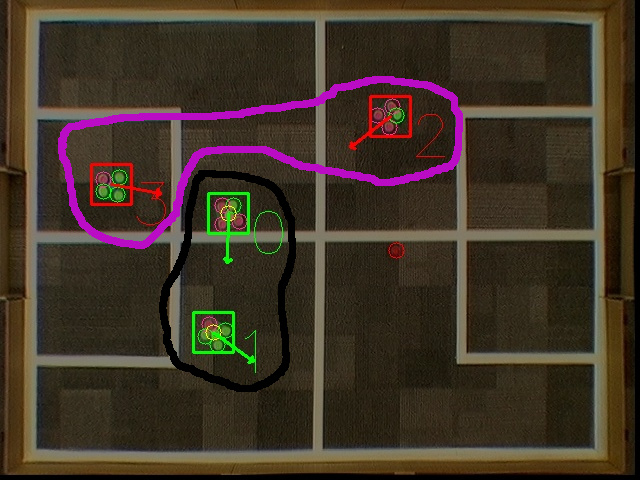
\includegraphics[height=60mm,width=90mm]{filter1.jpg}\newline\newline
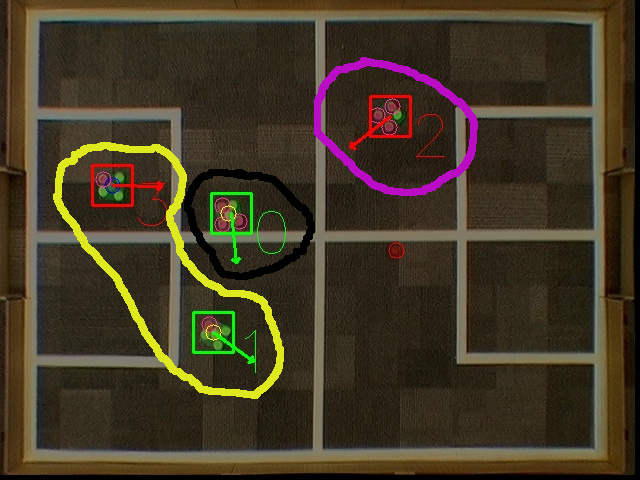
\includegraphics[height=60mm,width=90mm]{filter2.jpg}
\end{minipage}
\begin{minipage}{0.4\textwidth}
\mybox{black}{FILTER 1} $\{$ \tikz\draw[yellow,fill=yellow] (0, 0) circle (.5ex); \tikz\draw[pink,fill=pink] (0, 0) circle (.5ex); \tikz\draw[pink,fill=pink] (0, 0) circle (.5ex); \tikz\draw[pink,fill=pink] (0, 0) circle (.5ex); $\}$

To pass into here it must have a correct team spot and no other visible team color. It must also have three of its three spot color.

\bigskip

\mybox{yellow}{FILTER 2} $\{$ \tikz\draw[yellow,fill=yellow] (0, 0) circle (.5ex); \tikz\draw[pink,fill=pink] (0, 0) circle (.5ex); \tikz\draw[pink,fill=pink] (0, 0) circle (.5ex); \tikz\draw[pink,fill=pink] (0, 0) circle (.5ex); , \tikz\draw[yellow,fill=yellow] (0, 0) circle (.5ex); \tikz\draw[green,fill=green] (0, 0) circle (.5ex); $\}$ 

To pass into here it must have a correct team spot. It also must have more than one of its three spot color or less than two of its corner spot color.

\bigskip

\mybox{violet}{FILTER 3} $\{$ \tikz\draw[yellow,fill=yellow] (0, 0) circle (.5ex); \tikz\draw[pink,fill=pink] (0, 0) circle (.5ex); \tikz\draw[pink,fill=pink] (0, 0) circle (.5ex); \tikz\draw[pink,fill=pink] (0, 0) circle (.5ex); , \tikz\draw[yellow,fill=yellow] (0, 0) circle (.5ex); \tikz\draw[green,fill=green] (0, 0) circle (.5ex); , \tikz\draw[pink,fill=pink] (0, 0) circle (.5ex); \tikz\draw[pink,fill=pink] (0, 0) circle (.5ex); \tikz\draw[pink,fill=pink] (0, 0) circle (.5ex); $\}$  
 
To pass into here no team spot is required, it must only have more than one of its three spot color or less than two of its corner spot color.
\end{minipage}

\medskip

As each identity is found, its corresponding filters are blocked and its position is noted so that a robot does not get detected in the same place as the one that is already detected. Once any group of spots gets through a filter of a given identity, the identity of that robot is then updated using either the three spot or two spot method depending on what information is available. If a robot is not found, it keeps its original position. To handle cases where robots are lifted off the pitch, the system creates a ghost robot marked in blue on the vision feed. This tells the strategy to ignore the contribution to the game of that robot but the robot continues existing on the pitch in the vision thread.

\subsubsection{Finding the ball}

The algorithm looks for 10 red spots and checks through them in the order of descending area. To prevent a pink being misclassified as the ball, each red spot is checked whether it exists close to the centres of the robots. As the robots can shield the ball from view, a method is used which determines whether a specific robot is in range of the ball. If so, when the ball is shielded, an imaginary ball is placed along the orientation vector of that robot until the ball is found. This method is in place for all robots except for Venus because the sensor is being used instead to determine whether Venus has the ball.

\subsection{Strategy}

\subsubsection{Potential fields}

The strategy relies on the physical properties of a potential field. This makes it possible to compound together separate tasks that the robot has to undertake with ease, such as avoiding others and grabbing a ball, at the same time. Each interaction is implemented using the same behaviour as a charged electron would have when interacting with various physical objects of different charges. Using this it is possible to swerve in front of the kicks and navigate mazes of objects fast and efficiently. 

\subsubsection{State machine}

As seen in Table \ref{tab:machine} bla bla

\begin{table}[h!]
\centering
\begin{tabular}{ | l | l | }
\hline
\textbf{State} & \textbf{Trigger} \\ \hline
\texttt{FREE\_BALL\_YOURS} & \\ \hline
\texttt{ENEMY\_BALL\_TAKE\_PASS} &  \\ \hline
\texttt{ENEMY1\_BALL\_TAKE\_GOAL} &  \\ \hline
\texttt{ENEMY2\_BALL\_TAKE\_GOAL} &  \\ \hline
\texttt{FREE\_BALL\_NONE\_GOALSIDE} &  \\ \hline
\texttt{FREE\_BALL\_1\_GOALSIDE} &  \\ \hline
\texttt{FREE\_BALL\_2\_GOALSIDE} &  \\ \hline
\texttt{FREE\_BALL\_BOTH\_GOALSIDE} &  \\ \hline
\texttt{ATTACK\_PASS} &  \\ \hline
\texttt{ATTACK\_GOAL} &   \\ \hline
\texttt{RECEIVE\_PASS} &  \\ \hline
\end{tabular}
\caption{States available in the strategy system}
\label{tab:machine}
\end{table}

\subsubsection{State fields}

The following graphs were plotted using the command \texttt{map STATE\_NAME} which is ideal for visualisation and quick testing of newly defined fields. The graphs below contain quiver plots of the force acting on Venus at a given point in space. This is drawn on top of a heat map of the value of the potential field at a given point. 

\begin{minipage}{\linewidth}
\rule{\textwidth}{1pt}
\texttt{FREE\_BALL\_YOURS}\medskip

\begin{minipage}{0.5\textwidth}
\begin{center}
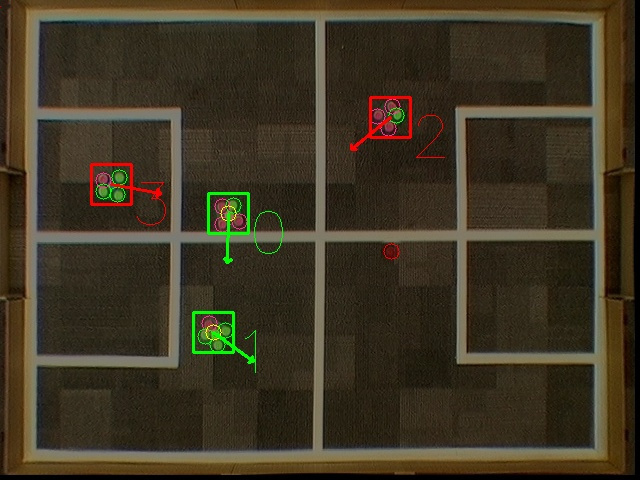
\includegraphics[height=40mm,width=50mm]{v3.jpg}\medskip
\end{center}

\textbf{Forces due to obstacles}:
The walls exert a force governed by a $1/r^3$ law on the pitch side of the wall where $r$ is the perpendicular distance to the wall. On the opposite side of the wall an attractive potential $-1/r^3$ is used instead to pull any robots into the pitch. An identical field is used in the penalty box, however, to avoid getting stuck in a local minima at the sides, the field inside the box pushes the robot to the front only and does not attract it back over the side it came from. As the box is finite, any position that is not perpendicular will exhibit a similar force, only $r$ will be the distance to the closest corner. The robots use a $1/r^2$ law where $r$ is the radial distance from the edge of the robot represented by the solid circle in red.
\end{minipage}
~
\begin{minipage}{0.5\textwidth}
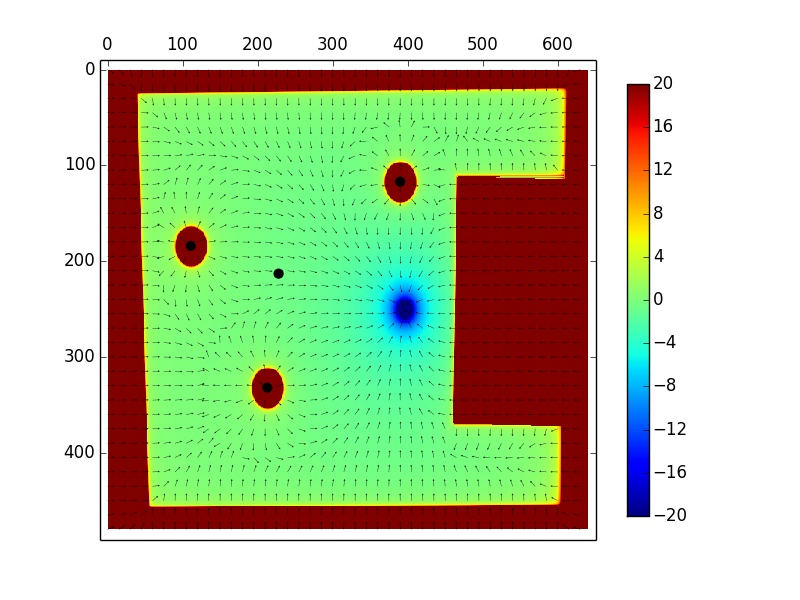
\includegraphics[height=70mm,width=100mm,trim=65 55 65 35,clip]{p3.jpg}\medskip

\textbf{Grabbing}: The ball uses an attractive radial field of $-1/r^2$. The amplitude of the field is larger than that of the robot to enable fast navigation. Once a potential of $-4$ is reached, the grab is initiated using quantised distance and angle motions enabled by the motor encoders. The $-4$ value has been chosen as it implies the ball is clear of any obstacles as otherwise the potential value would be higher.
\end{minipage}
\end{minipage}\medskip

\begin{minipage}{\linewidth}
\rule{\textwidth}{1pt}
\texttt{ENEMY\_BALL\_TAKE\_PASS}\medskip

\begin{minipage}{0.5\textwidth}
\begin{center}
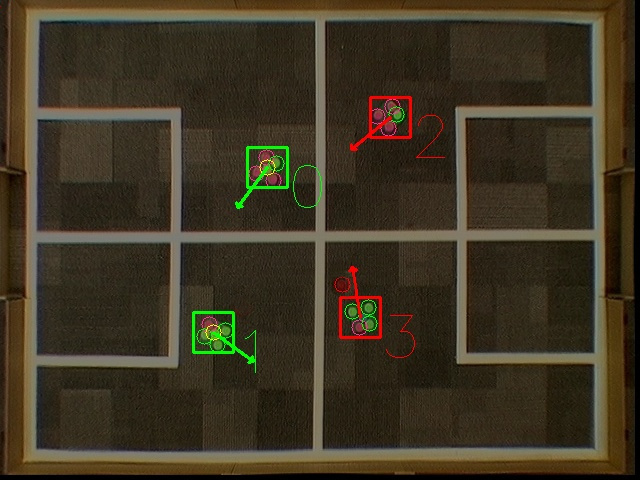
\includegraphics[height=40mm,width=50mm]{v1_2.jpg}\medskip
\end{center}

\textbf{Blocking pass}: A finite axial field is used to enable smooth motion during the block of a pass from any point in the pitch. The points in question are first rotated so that the field is flush with the x-axis and the force is calculated using the following equation and rotated back. $d$ is the perpendicular distance, $a$ is the parallel distance to the end with the smaller $x$ value and $b$ is similar dimension in the exact opposite direction.

$\left(\frac{1}{\sqrt{b^2 + d^2}}-\frac{1}{\sqrt{a^2 + d^2}},\frac{b}{d\sqrt{b^2 + d^2}}+\frac{a}{d\sqrt{a^2 + d^2}}\right)$
\end{minipage}
~
\begin{minipage}{0.5\textwidth}
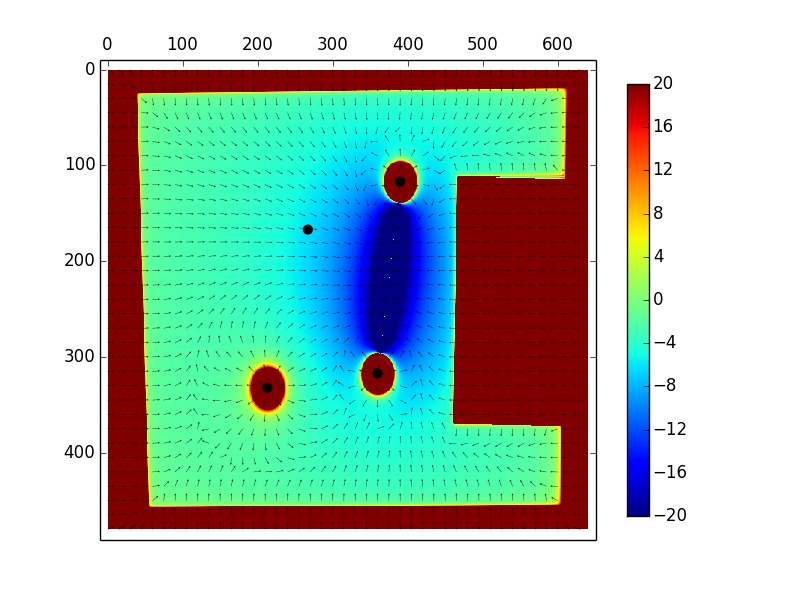
\includegraphics[height=70mm,width=100mm,trim=65 55 65 35,clip]{p1.jpg}\medskip

\textbf{Interceptions}: When the current potential of Venus reaches $-12$, the block is satisfactory and the robot faces the ball with its grabber open. When the ball is shot as it is moving, the \texttt{FREE\_BALL\_YOURS} state is activated causing an attraction to the moving ball.
\end{minipage}
\end{minipage}\medskip

\begin{minipage}{\linewidth}
\rule{\textwidth}{1pt}
\texttt{ENEMY2\_BALL\_TAKE\_GOAL} $_{\text{(\texttt{ENEMY1\_BALL\_TAKE\_GOAL})}}$\medskip

\begin{minipage}{0.5\textwidth}
\begin{center}
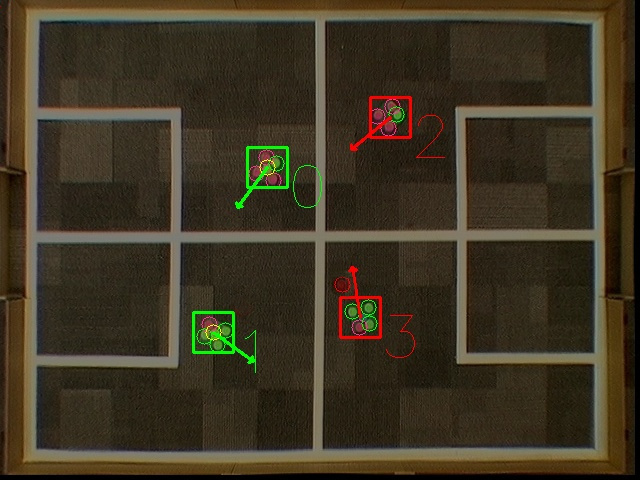
\includegraphics[height=40mm,width=50mm]{v1_2.jpg}\medskip
\end{center}

\textbf{Blocking goal}: The same field is used from the state above but for a block between the goal and an enemy robot. The current satisfactory potential for this block is $-14$ in order to be sure to block the whole goal.
\end{minipage}
~
\begin{minipage}{0.5\textwidth}
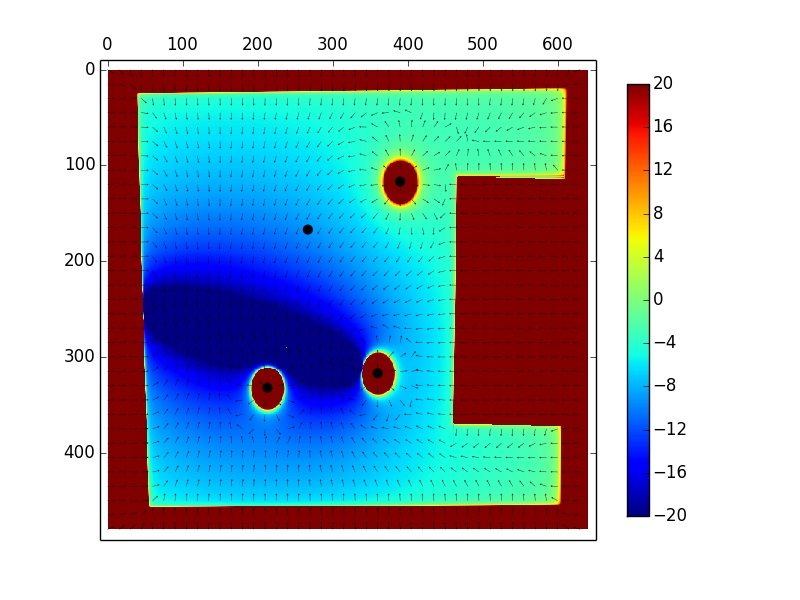
\includegraphics[height=70mm,width=100mm,trim=65 55 65 35,clip]{p2.jpg}\medskip
\end{minipage}
\end{minipage}\medskip

\begin{minipage}{\linewidth}
\rule{\textwidth}{1pt}
\texttt{FREE\_BALL\_NONE\_GOALSIDE} $_{\text{(\texttt{FREE\_BALL\_1\_GOALSIDE}, \texttt{FREE\_BALL\_2\_GOALSIDE})}}$\medskip

\begin{minipage}{0.5\textwidth}
\begin{center}
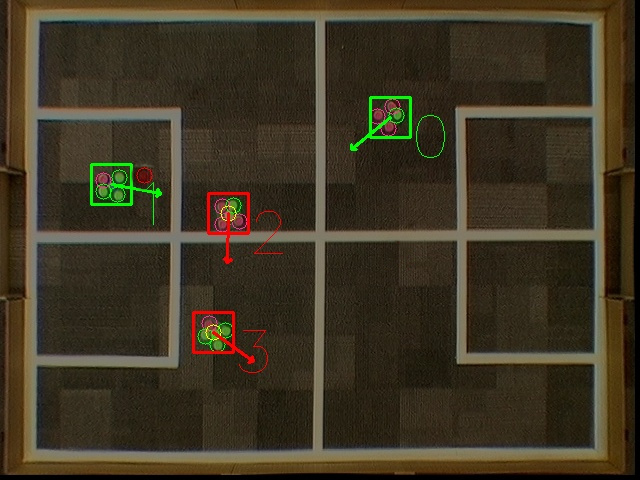
\includegraphics[height=40mm,width=50mm]{v4.jpg}\medskip
\end{center}

\textbf{Optimising position}: Given your team mate is either fetching or has the ball you want to find the best position to receive a pass. Two fields are added in order to implement this: \begin{enumerate} \item The shadowed array blocking the pass. \item The shadowed array blocking the goal. \end{enumerate} This state represents a double blocked pass. An identical type of field is used in the defence states, however, one end is placed at the start of the shadow and the other three pitch lengths away. This is so that Venus is repelled perpendicular to the shadow and also parallel around the enemy robots if needs be.
\end{minipage}
~
\begin{minipage}{0.5\textwidth}
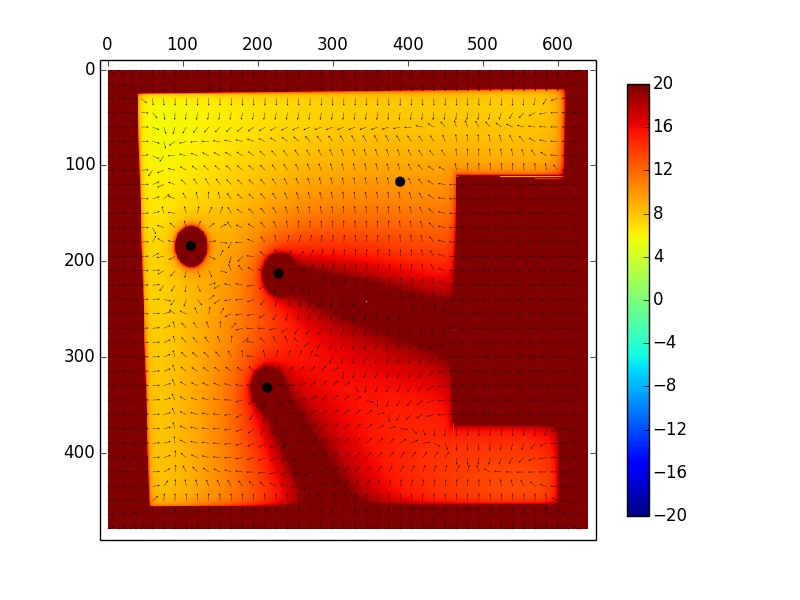
\includegraphics[height=70mm,width=100mm,trim=65 55 65 35,clip]{p4.jpg}\medskip

Once a satisfactory potential of 6 is reached, Venus will turn and wait to except the pass. As the other robots move, Venus will keep trying to minimise his potential until a value of 6 is obtained.
\end{minipage}
\end{minipage}\medskip

\begin{minipage}{\linewidth}
\rule{\textwidth}{1pt}
\texttt{FREE\_BALL\_BOTH\_GOALSIDE} $_{\text{(\texttt{FREE\_BALL\_1\_GOALSIDE}, \texttt{FREE\_BALL\_2\_GOALSIDE})}}$\medskip

\begin{minipage}{0.5\textwidth}
\begin{center}
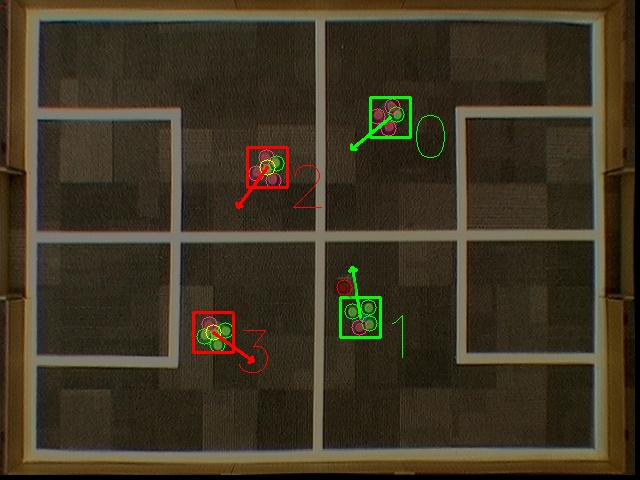
\includegraphics[height=40mm,width=50mm]{v5.jpg}\medskip
\end{center}

\textbf{Local minima}: Whilst optimising position Venus can get stuck as enemy players close up to defend the same shot. To deal with this, a timer is used so that if Venus has been sitting in a unsatisfactory potential for too long, we remove the least import field. In this case, the furthest player blocking the goal.
\end{minipage}
~
\begin{minipage}{0.5\textwidth}
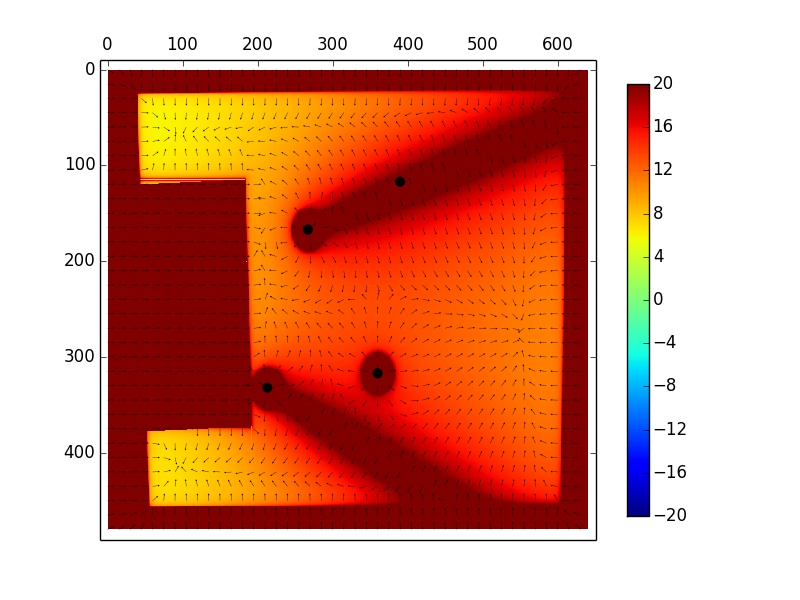
\includegraphics[height=70mm,width=100mm,trim=65 55 65 35,clip]{p5.jpg}\medskip

\textbf{Handling opponents that divide up defensive positions}: As outlined in the state above, this graph represents a double blocked goal and the final two states that are not shown are a mixture of this state and the state above.
\end{minipage}
\end{minipage}

\rule{\textwidth}{1pt}

\section{Sensors}
\subsection{Rotary encoder board}

Each NXT motor is connected to the rotary encoder board which is depicted in Figure \ref{fig:rotary}. The connections in the anticlockwise order from the top are: the I2C bus to the Arduino, back right motor, back left motor, front left motor, and front right motor. Using this board the information about the amount of rotations the motor has performed since the last query is available for the Arduino code as a separate integer for every motor. Every 5 ms the board is queried whether the target value has been reached. After the average of the rotary values of all four motors becomes greater or equal to the target value, the motors are stopped.

\begin{figure}[ht!]
\centering
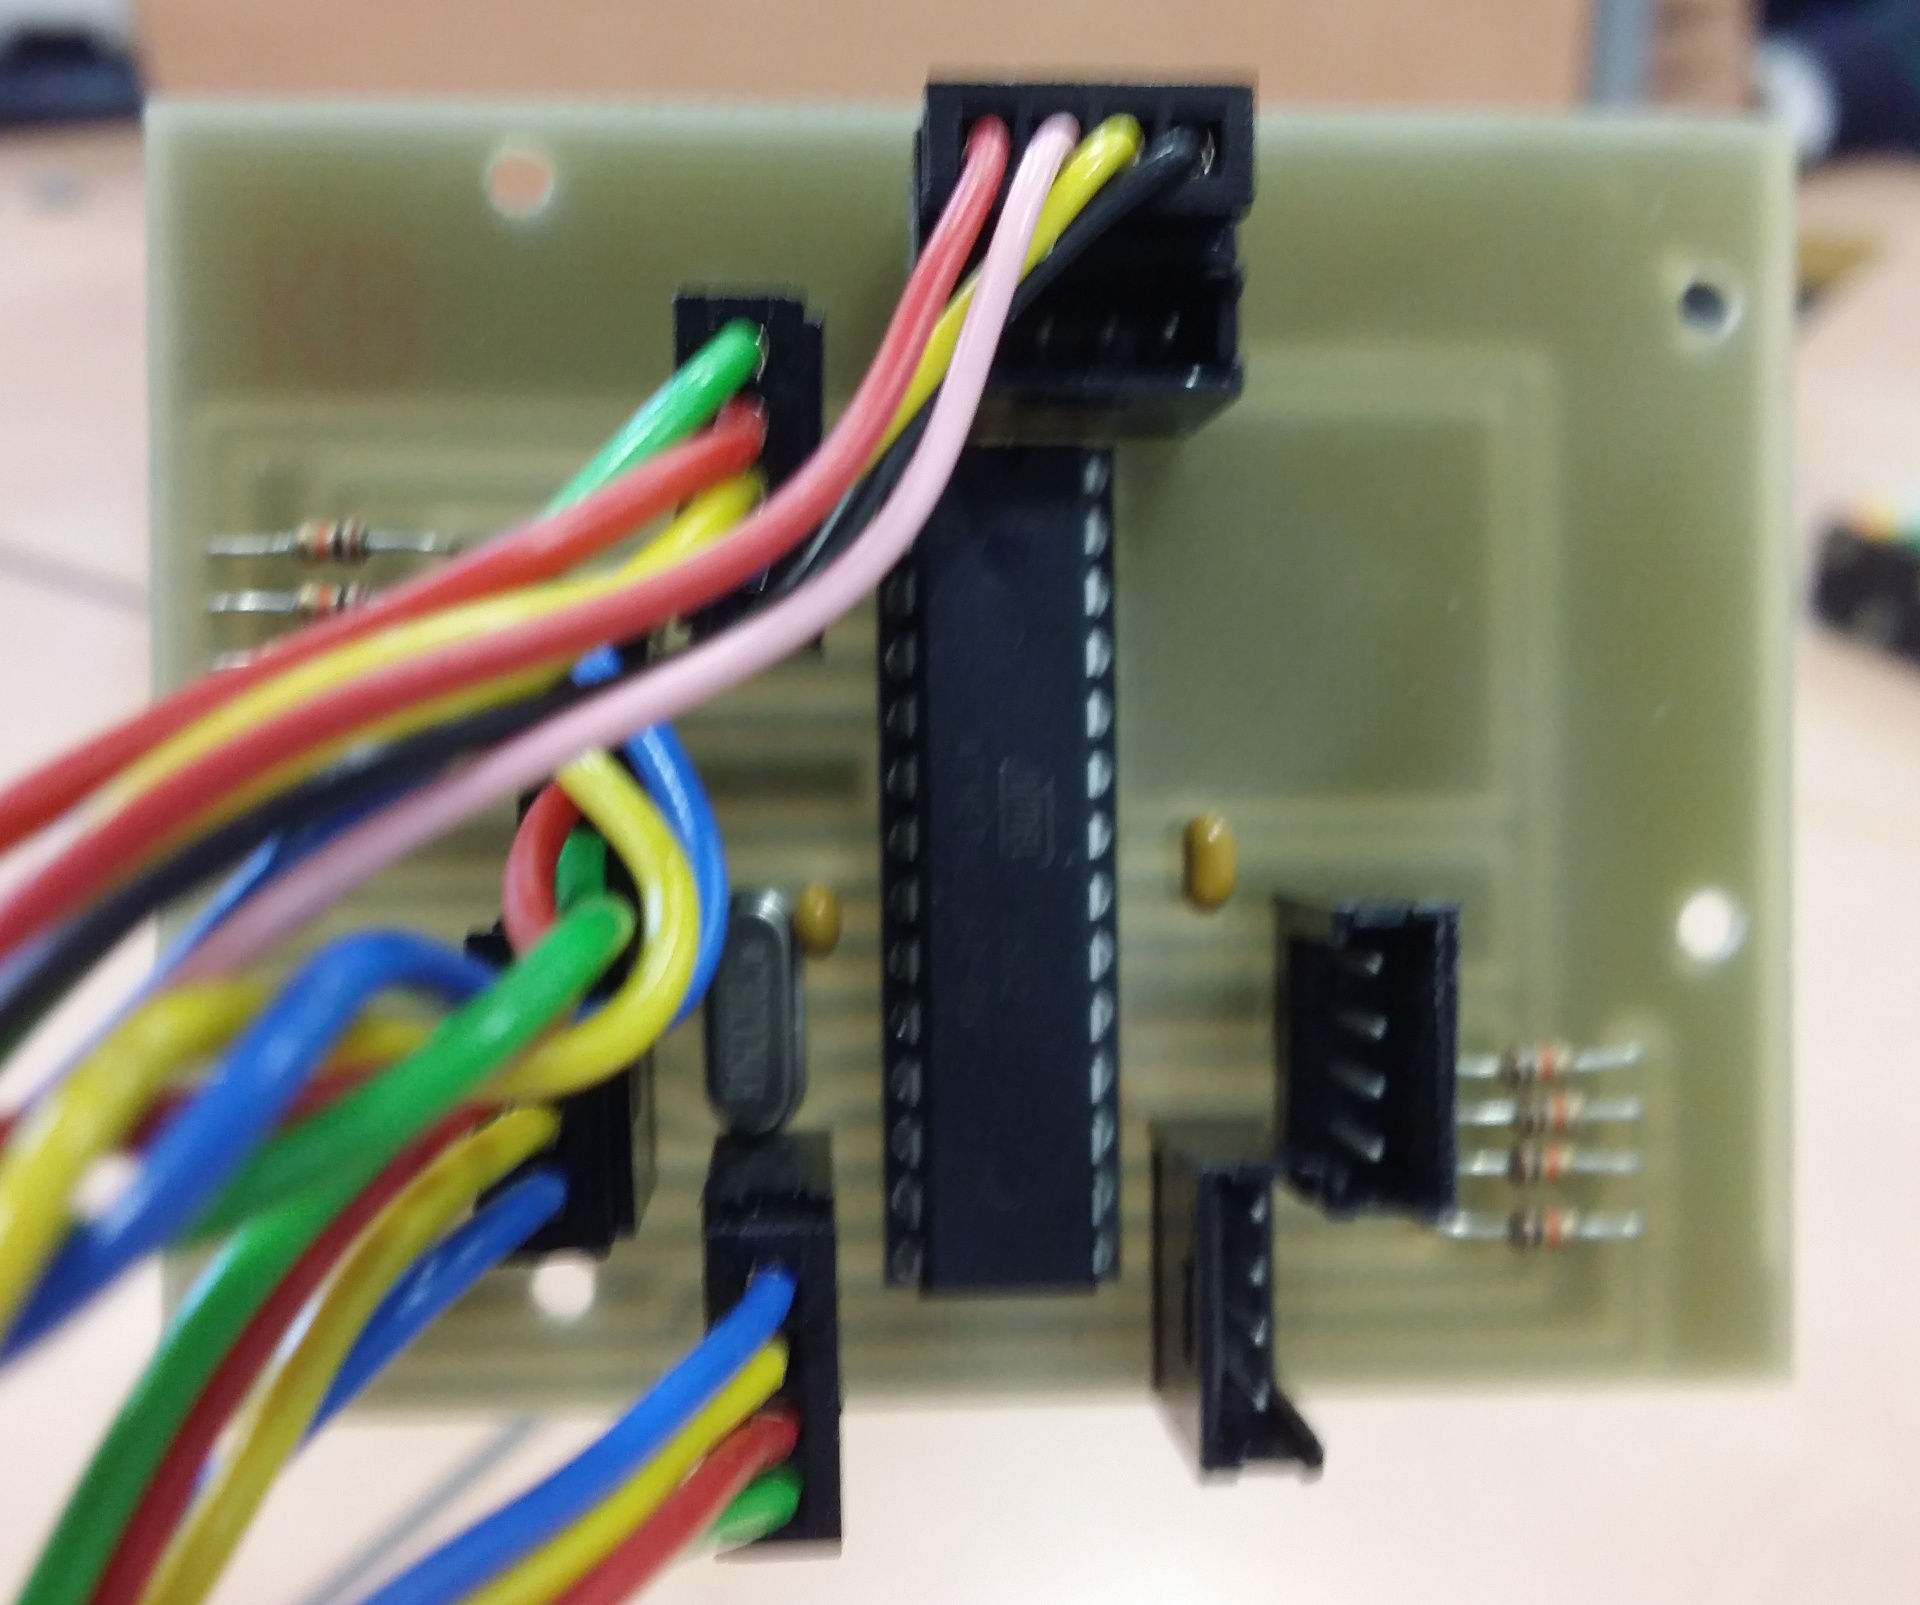
\includegraphics[scale=.1]{rotary1}
\caption{The rotary encoder board}
\label{fig:rotary}
\end{figure}

\subsection{Light sensor}

The light sensor is located above the grabber as seen in Figure \ref{fig:sensor}. It is used to check whether
the robot has successfully acquired the ball after grabbing. The sensor
provides an integer value that increases the greater the distance to the
nearest object in its direct line of sight is. Then the Arduino compares the integer
to a predefined threshold corresponding to the red ball. Sometimes a white
line inside the pitch can be mistaken for the ball due to their similar sensor
values. An IR sensor was also tested and its returned values were deemed less reliable than
those of the light sensor.

\begin{figure}[ht!]
\centering
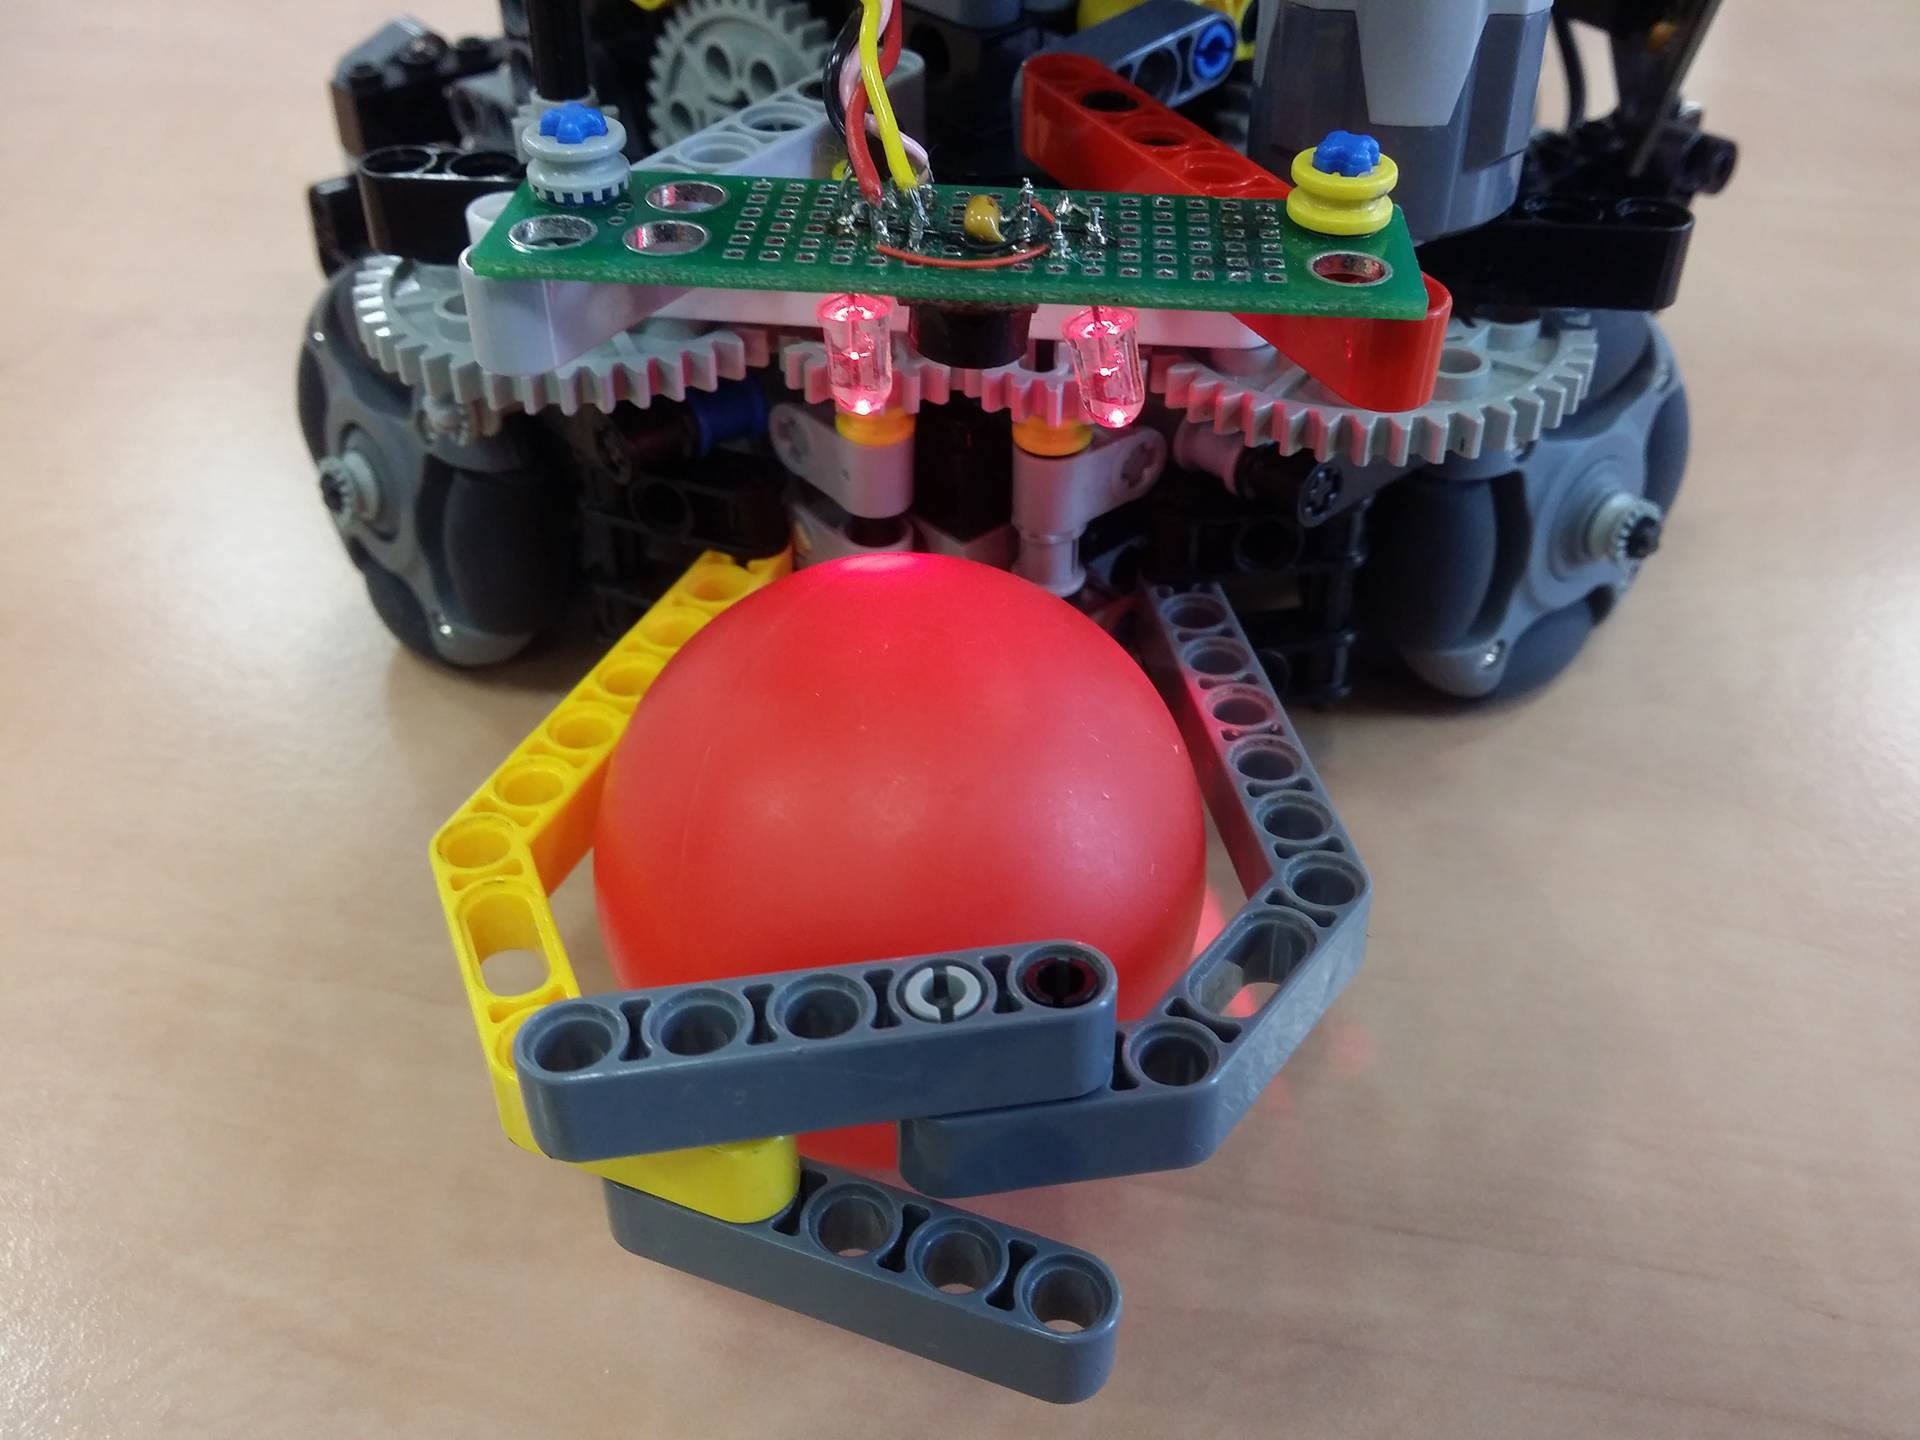
\includegraphics[scale=.1]{sensor1}
\caption{The light sensor with the ball grabbed}
\label{fig:sensor}
\end{figure}

\end{document}
